\documentclass[12pt,a4paper]{article}

\usepackage[utf8]{inputenc}
\usepackage[vietnamese]{babel}
\usepackage{amsmath, amssymb, amsfonts}
\usepackage{graphicx}
\usepackage{booktabs}
\usepackage{tabularx}
\usepackage{multirow}
\usepackage{hyperref}
\usepackage{cite}
\usepackage{geometry}
\usepackage{xcolor}
\usepackage{microtype}
\usepackage{float}
\usepackage{caption}
\usepackage{subcaption}

\geometry{
    a4paper,
    left=30mm,
    right=20mm,
    top=25mm,
    bottom=25mm
}

\hypersetup{
    colorlinks=true,
    linkcolor=blue!70!black,
    citecolor=red!70!black,
    urlcolor=blue!80!black
}

\title{
    \Large \textbf{ĐẠI HỌC QUỐC GIA TP. HỒ CHÍ MINH} \\
    \textbf{TRƯỜNG ĐẠI HỌC CÔNG NGHỆ THÔNG TIN} \\
    \textbf{KHOA MẠNG MÁY TÍNH VÀ TRUYỀN THÔNG} \\[1.5cm]
    \LARGE \textbf{BÁO CÁO TIẾN ĐỘ \& KẾT QUẢ THỰC NGHIỆM KHÓA LUẬN TỐT NGHIỆP} \\[0.5cm]
    \Large \textbf{XÂY DỰNG VÀ ĐÁNH GIÁ PROTOTYPE HỆ THỐNG PHÁT HIỆN XÂM NHẬP IOT SỬ DỤNG FEDERATED LEARNING TRONG MÔI TRƯỜNG DỮ LIỆU NON-IID}
}

\author{
    \textbf{Sinh viên thực hiện:} Nguyễn Việt Kỳ Quân -- 23521267 \\
    \textbf{Cán bộ hướng dẫn:} PGS. TS. Lê Trung Quân \\[0.5cm]
    \textit{Chuyên ngành: Mạng máy tính và An toàn thông tin}
}

\date{\today}

\begin{document}

\maketitle
\thispagestyle{empty}
\newpage

\begin{abstract}
Sự phát triển mạnh mẽ của Internet vạn vật (IoT) đã mở rộng đáng kể bề mặt tấn công mạng, đòi hỏi các giải pháp Phát hiện Xâm nhập (NIDS) hiệu quả và bảo toàn quyền riêng tư. Học liên đoàn (Federated Learning -- FL) nổi lên như một hướng tiếp cận đầy triển vọng cho phép huấn luyện mô hình phân tán mà không cần tập trung hóa dữ liệu thô. Tuy nhiên, sự phi đồng nhất về mặt thống kê (Non-IID) và hiện tượng mất cân bằng lớp cực đoan giữa các trạm mạng IoT biên đặt ra rào cản kỹ thuật nghiêm trọng đối với quá trình hội tụ mô hình. Báo cáo này trình bày thiết kế, hiện thực nguyên mẫu (prototype) và đánh giá thực nghiệm đa chiều của hệ thống FL-IoT-IDS trên tập dữ liệu chuẩn mới CICIoT2023. Hệ thống được triển khai trên nền tảng giao thức Flower gRPC sockets với mô hình Tabular MLP nhỏ gọn (~14,024 tham số, ~54.28 KB). Thông qua chuỗi 9 kịch bản thực nghiệm có kiểm soát (từ E2 đến E6) bao gồm cả dữ liệu IID và phân phối Dirichlet Non-IID ($\alpha \in \{1.0, 0.5, 0.1\}$), nghiên cứu cung cấp các bằng chứng thực nghiệm phản biện định lượng: (1) Chỉ ra giới hạn toán học của cơ chế trung bình trọng số trong FedAvg và số hạng điều hòa FedProx khi xử lý các lớp tấn công thiểu số cực hiếm ($<0.5\%$ như Web-based với tỷ lệ nhận diện Recall $<2\%$); (2) Xác định đường cong suy thoái định lượng của Macro-F1 khi hệ số $\alpha$ giảm dần; và (3) Đánh giá chi phí truyền thông mạng thực tế khi mở rộng quy mô từ 5 lên 10 clients. Báo cáo phản ánh trung thực kết quả thực nghiệm, đóng góp khung benchmark chuẩn xác cho các nghiên cứu tiếp theo.
\end{abstract}

\textbf{Từ khóa:} Học liên đoàn, Phát hiện xâm nhập IoT, Non-IID, Phân phối Dirichlet, FedAvg, FedProx, CICIoT2023, Flower gRPC.

\newpage
\tableofcontents
\newpage

% ==============================================================================
% CHƯƠNG 1
% ==============================================================================
\section{Giới thiệu và Đặt vấn đề}
\label{sec:intro}

\subsection{Bối cảnh và Động lực Nghiên cứu}
Sự bùng nổ của các thiết bị Internet of Things (IoT) đã tạo ra một hệ sinh thái mạng phức tạp với hàng tỷ kết nối thông minh. Mặc dù mang lại tiện ích to lớn, phần lớn các thiết bị IoT biên (Edge IoT) đều có tài nguyên tính toán hạn chế, khả năng bảo mật yếu và thường xuyên trở thành mục tiêu của các chiến dịch tấn công diện rộng như từ chối dịch vụ phân tán (DDoS/DoS), mạng máy tính ma Mirai, hay dò quét mật khẩu (Brute-force) \cite{neto2023ciciot2023}. Để bảo vệ hạ tầng mạng IoT, các Hệ thống Phát hiện Xâm nhập Mạng (NIDS) ứng dụng Học máy (ML) và Học sâu (DL) đóng vai trò then chốt \cite{huang2022federated}.

Trong mô hình học máy tập trung truyền thống (Centralized ML), toàn bộ lưu lượng mạng từ các thiết bị phân tán bắt buộc phải gửi về một máy chủ trung tâm để huấn luyện. Cách tiếp cận này bộc lộ hai yếu điểm chí mạng: (1) Vi phạm nghiêm trọng quyền riêng tư dữ liệu theo các quy định an toàn thông tin hiện đại; và (2) Tiêu tốn băng thông đường truyền khổng lồ, gây nghẽn cổ chai tại gateway trung tâm \cite{yang2019federated}.

\subsection{Các Thách thức Cốt lõi của Mạng IoT}
Học liên đoàn (Federated Learning -- FL) do McMahan et al. \cite{mcmahan2017communication} đề xuất đã mở ra hướng đi mới: các trạm biên tự huấn luyện mô hình trên dữ liệu cục bộ và chỉ chia sẻ các tham số trọng số ($\mathbf{w}$) về máy chủ điều phối. Tuy nhiên, việc áp dụng FL vào bài toán an ninh mạng IoT gặp phải ba rào cản kỹ thuật nghiêm trọng:
\begin{enumerate}
    \item \textbf{Dữ liệu phi đồng nhất (Non-IID Data Heterogeneity):} Trong thế giới thực, các trạm IoT biên quan sát lưu lượng mạng rất khác biệt tùy thuộc vào vị trí vật lý và chức năng thiết bị. Sự khác biệt phân phối nhãn dẫn đến hiện tượng trôi dạt trọng số cục bộ (\textit{Client Drift}), khiến thuật toán Federated Averaging (FedAvg) suy thoái nặng nề hoặc không thể hội tụ \cite{li2020federated, hsu2019measuring}.
    \item \textbf{Mất cân bằng lớp cực đoan (Severe Structural Class Imbalance):} Trong các tập dữ liệu lưu lượng mạng như CICIoT2023, các cuộc tấn công DDoS/DoS chiếm hơn $70\%$ lưu lượng, trong khi các cuộc tấn công tinh vi nguy hiểm như Web-based (SQL Injection, XSS) hay Brute-force chỉ chiếm dưới $0.5\%$. Khi huấn luyện phân tán, các lớp đa số áp đảo hoàn toàn tín hiệu gradient, khiến mô hình gần như mất khả năng nhận diện các mối đe dọa thiểu số \cite{alahmari2025enhancing}.
    \item \textbf{Giới hạn phần cứng thiết bị biên (Resource Constraints):} Các gateway biên chỉ sở hữu năng lực CPU khiêm tốn và bộ nhớ hạn hẹp, không thể gánh vác các kiến trúc học sâu cồng kềnh (CNN-LSTM, Transformer) vốn đòi hỏi hàng chục megabytes payload cho mỗi vòng giao tiếp \cite{albanbay2025federated}.
\end{enumerate}

\subsection{Mục tiêu và Định vị Đóng góp của Đề tài}
Bám sát định hướng trong Đề cương chi tiết khóa luận tốt nghiệp, đề tài này không đặt mục tiêu đề xuất một thuật toán tối ưu toán học hoàn toàn mới. Thay vào đó, đề tài tập trung vào tính \textbf{hiện thực hóa kỹ thuật} và \textbf{đo kiểm thực nghiệm có hệ thống (Empirical & Benchmarking Study)} nhằm cung cấp ba đóng góp thực chất:
\begin{itemize}
    \item \textbf{Xây dựng hoàn chỉnh Prototype FL-IoT-IDS:} Hiện thực hóa kiến trúc 4 lớp dựa trên framework Flower \cite{beutel2020flower} giao tiếp qua socket TCP/IP gRPC thực thụ, sử dụng mô hình Tabular MLP nhỏ gọn (~14,024 tham số, ~54.28 KB) vận hành tối ưu trên CPU thiết bị biên.
    \item \textbf{Phát hiện thực nghiệm phản biện (Negative Finding):} Chứng minh định lượng rằng các cơ chế trung bình trọng số thông thường trong FedAvg/FedProx không thể giải quyết được bài toán phát hiện tấn công cực hiếm ($<0.5\%$), cung cấp bằng chứng thực tế về giới hạn của FL trong an ninh mạng.
    \item \textbf{Ma trận đối sánh đa chiều chuẩn mực:} Thiết lập chuỗi kịch bản có kiểm soát từ E2 đến E6, vạch ra đường cong suy thoái định lượng theo hệ số Dirichlet $\alpha \in \{1.0, 0.5, 0.1\}$ và đánh giá chi phí truyền thông khi mở rộng quy mô $K \in \{5, 7, 10\}$ trạm biên.
\end{itemize}

% ==============================================================================
% CHƯƠNG 2
% ==============================================================================
\section{Cơ sở Lý thuyết và Tổng quan Nghiên cứu Liên quan}
\label{sec:literature}

\subsection{Tập Dữ liệu Chuẩn CICIoT2023}
Tập dữ liệu CICIoT2023 \cite{neto2023ciciot2023} được thu thập tại Viện An ninh mạng Canada (CIC), mô phỏng môi trường mạng IoT quy mô lớn với 105 thiết bị phần cứng thật. Bộ dữ liệu chứa hơn 47 triệu bản ghi lưu lượng mạng flow-based với 39 đặc trưng số (statistical network flow features) và 33 phân loại tấn công được gom nhóm thành 8 lớp chính: \textit{Benign, Brute-force, DDoS, DoS, Mirai, Reconnaissance, Spoofing}, và \textit{Web-based}. CICIoT2023 phản ánh chính xác sự mất cân bằng thực tế của lưu lượng mạng IoT hiện đại.

\subsection{Thuật toán FedAvg và Thách thức Non-IID}
Thuật toán Federated Averaging (FedAvg) \cite{mcmahan2017communication} thực hiện tổng hợp tham số mô hình toàn cục sau mỗi round $t$ dựa trên tỷ lệ số lượng mẫu dữ liệu cục bộ $n_k$ của $K$ trạm biên tham gia:
\begin{equation}
    \mathbf{w}_{t+1} = \sum_{k=1}^K \frac{n_k}{N} \mathbf{w}_{t+1}^{(k)} \quad \text{với} \quad N = \sum_{k=1}^K n_k
    \label{eq:fedavg}
\end{equation}
Trong môi trường IID, FedAvg hội tụ nhanh chóng. Tuy nhiên, khi dữ liệu phân tán bị lệch phân phối (Non-IID), mục tiêu tối ưu cục bộ $F_k(\mathbf{w})$ của từng client bị phân kỳ so với mục tiêu toàn cục $F(\mathbf{w})$. Khoảng cách giữa các vector nghiệm cục bộ tạo ra hiện tượng trôi dạt tham số (\textit{Client Drift}):
\begin{equation}
    \Delta \mathbf{w}^{(k)} = \|\mathbf{w}_{\text{local}}^{(k)} - \mathbf{w}_{\text{global}}^{(t)}\|_2 = \sqrt{\sum_{l} \|\mathbf{w}_{\text{local}}^{(k, l)} - \mathbf{w}_{\text{global}}^{(t, l)}\|_2^2}
    \label{eq:drift}
\end{equation}

\subsection{Thuật toán FedProx và Điều hòa Khoảng cách}
Để đối phó với hiện tượng trôi dạt tham số do Non-IID, Li et al. \cite{li2020federated} đề xuất thuật toán FedProx, bổ sung một số hạng phạt điều hòa (proximal term) vào hàm mất mát cục bộ của mỗi client:
\begin{equation}
    \min_{\mathbf{w}} h_k(\mathbf{w}; \mathbf{w}_t) = F_k(\mathbf{w}) + \frac{\mu}{2} \|\mathbf{w} - \mathbf{w}_t\|_2^2
    \label{eq:fedprox}
\end{equation}
Trong đó $\mu \ge 0$ là hệ số điều hòa. Thành phần phạt $\frac{\mu}{2}\|\mathbf{w} - \mathbf{w}_t\|_2^2$ có tác dụng "buộc dây" (anchor) vector trọng số của client không bị trôi dạt quá xa khỏi mô hình toàn cục $\mathbf{w}_t$, giúp quá trình hội tụ ổn định hơn khi dữ liệu giữa các client có sự dị biệt lớn.

\subsection{Mô hình hóa Non-IID bằng Phân phối Dirichlet}
Theo phương pháp luận chuẩn của Hsu et al. \cite{hsu2019measuring}, tính phi đồng nhất về nhãn được mô phỏng thông qua phân phối Dirichlet:
\begin{equation}
    \mathbf{p}_c \sim \text{Dir}(\alpha \cdot \mathbf{1}_K)
\end{equation}
Trong đó $\mathbf{p}_c$ là vector xác suất phân bổ mẫu của lớp tấn công $c$ cho $K$ client, và $\alpha > 0$ là tham số tập trung (concentration parameter). Khi $\alpha \to \infty$, phân phối tiến về IID; khi $\alpha \to 0$, dữ liệu bị phân mảnh cực đoan, mỗi trạm biên chỉ chứa một vài lớp duy nhất.

\subsection{Đối sánh với các Công trình Công bố Gần đây (2024 -- 2026)}
Bảng \ref{tab:lit_comparison} tổng hợp định vị học thuật của đề tài so với các công trình nghiên cứu tiêu biểu giai đoạn 2024 -- 2026 trên tập dữ liệu CICIoT2023.

\begin{table}[H]
\centering
\caption{Đối sánh công trình này với các nghiên cứu FL-IoT-IDS giai đoạn 2024 -- 2026.}
\label{tab:lit_comparison}
\small
\begin{tabularx}{\textwidth}{l p{4.2cm} p{4.5cm} X}
\toprule
\textbf{Công trình} & \textbf{Mô hình \& Thuật toán} & \textbf{Xử lý Dữ liệu \& Phân vùng} & \textbf{Hạn chế chưa giải quyết} \\
\midrule
Alahmari et al. (2025) \cite{alahmari2025enhancing} & Deep Neural Network, FedAvg & Sử dụng mạng đối kháng GANs để sinh dữ liệu nhân tạo & Không khả thi trong mạng phân tán thực; không đo Client Drift. \\
Albanbay et al. (2025) \cite{albanbay2025federated} & CNN / MLP, FedAvg & Khảo sát scaling dữ liệu trên CICIoT2023 & Chỉ thử nghiệm 1 mốc $\alpha$ cố định; bỏ qua chi phí truyền thông. \\
Huang et al. (2022) \cite{huang2022federated} & MLP / FedAvg & Phân vùng Non-IID trên dataset cũ & Mô hình cũ; không đánh giá tấn công thiểu số. \\
\textbf{Công trình này (FL-IoT-IDS)} & \textbf{TabularIoTMLP (14k params), FedAvg vs FedProx} & \textbf{3 mốc Dirichlet ($\alpha \in \{1.0, 0.5, 0.1\}$), No-leakage RobustScaler} & \textbf{Đo toàn diện: Macro-F1, Minority Recall, Client Drift, Comm Cost, Scale $K \in \{5, 7, 10\}$.} \\
\bottomrule
\end{tabularx}
\end{table}

% ==============================================================================
% CHƯƠNG 3
% ==============================================================================
\section{Thiết kế Kiến trúc Hệ thống Prototype FL-IoT-IDS}
\label{sec:system_design}

\subsection{Tổng quan Kiến trúc 4 Lớp (The 4-Layer Architecture)}
Hệ thống prototype FL-IoT-IDS được thiết kế theo cấu trúc mô-đun 4 lớp chặt chẽ nhằm bảo đảm tính độc lập dữ liệu và khả năng tái lập thực nghiệm:
\begin{enumerate}
    \item \textbf{Lớp 1 -- Dữ liệu và Phân vùng (Data \& Partitioning Layer):} Thực hiện chuẩn hóa đặc trưng bằng RobustScaler (chỉ fit trên tập train), phân chia thành $70\%$ dữ liệu liên đoàn và $30\%$ dữ liệu kiểm định tương lai (Upcoming / Unseen Data). Dữ liệu liên đoàn được chia cho $K$ client theo Stratified IID hoặc Dirichlet Non-IID.
    \item \textbf{Lớp 2 -- Trạm Giám sát IoT Biên (Federated Edge Client Layer):} Mỗi client vận hành một mô hình \texttt{TabularIoTMLP} gồm 3 tầng tuyến tính kết hợp hàm kích hoạt ReLU và Dropout ($20\%$):
    $$\text{Linear}(39, 128) \to \text{ReLU} \to \text{Dropout} \to \text{Linear}(128, 64) \to \text{ReLU} \to \text{Linear}(64, 8)$$
    Tổng số lượng tham số là 14,024 tham số, tương đương kích thước lưu trữ $54.28\text{ KB}$, hoàn toàn tương thích với bộ nhớ RAM dưới 1 MB của thiết bị IoT biên.
    \item \textbf{Lớp 3 -- Máy chủ Điều phối và Tổng hợp (Federated Server Layer):} Vận hành trên framework Flower kết nối qua gRPC sockets. Máy chủ điều khiển chiến lược tổng hợp (FedAvg hoặc FedProx) và cơ chế lưu trữ trọng số tối ưu \texttt{best\_weights.npz} dựa trên Macro-F1.
    \item \textbf{Lớp 4 -- Khung Đánh giá và Đo lường Đa chiều (Evaluation \& Monitoring Layer):} Giám sát song song cả chất lượng mô hình (Macro-F1, Minority Recall, Confusion Matrix) và chỉ số mạng phân tán (Chi phí truyền thông $2\sum m_t B$, Client Drift $\Delta \mathbf{w}$).
\end{enumerate}

\subsection{Công thức Ước lượng Chi phí Truyền thông}
Theo đặc tả tại Mục 9 của Đề cương chi tiết, tổng chi phí truyền thông tích lũy hai chiều qua mạng được xác định bởi công thức:
\begin{equation}
    \text{CommCost} = 2 \times \sum_{t=1}^T m_t \cdot B
    \label{eq:comm_cost}
\end{equation}
Trong đó $T$ là tổng số round giao tiếp, $m_t$ là số trạm biên tham gia tại round $t$, $B$ là dung lượng mô hình ($B = 54.28\text{ KB}$), và hệ số $2$ phản ánh chi phí truyền tải hai chiều (server gửi mô hình toàn cục xuống client và client gửi cập nhật trọng số lên server).

% ==============================================================================
% CHƯƠNG 4
% ==============================================================================
\section{Kết quả Thực nghiệm và Phân tích Chuyên sâu}
\label{sec:experiments}

\subsection{Thiết lập Môi trường và Ma trận Benchmark}
Tất cả các kịch bản thực nghiệm được cấu hình đồng nhất với số vòng giao tiếp $T=10$, số epoch cục bộ $E=2$, kích thước batch $64$, tốc độ học $\eta = 10^{-3}$ với bộ tối ưu AdamW. Mô hình toàn cục tốt nhất được đánh giá trên cùng một tập \textbf{Global Test Set độc lập ($30\%$ Upcoming Data)} với 1,535,000 mẫu kiểm định.

\subsection{Bảng Tổng hợp Kết quả Thực nghiệm Master Benchmark}
Bảng \ref{tab:master_benchmark} trình bày toàn bộ số liệu thực nghiệm thu thập từ 9 kịch bản phân tán đã hoàn thành trong hệ thống.

\begin{table}[H]
\centering
\caption{Bảng Master Benchmark kết quả thực nghiệm hệ thống FL-IoT-IDS trên CICIoT2023.}
\label{tab:master_benchmark}
\small
\begin{tabularx}{\textwidth}{l c c c c c c}
\toprule
\textbf{Kịch bản Thực nghiệm (Scenario)} & \textbf{Accuracy} & \textbf{Macro-F1} & \textbf{Web-based} & \textbf{Brute-force} & \textbf{Comm Cost} & \textbf{Drift} \\
& \textbf{(\%)} & \textbf{(\%)} & \textbf{Recall (\%)} & \textbf{Recall (\%)} & \textbf{(MB)} & \textbf{L2 Norm} \\
\midrule
\multicolumn{7}{l}{\textit{Nhóm Kịch bản E2: Môi trường IID Cơ sở ($K=5$)}} \\
\texttt{flower\_e2\_fedavg\_iid} & \textbf{84.60} & \textbf{68.00} & \textbf{1.66} & \textbf{20.57} & 5.30 & 10.21 \\
\texttt{flower\_e2\_fedprox\_mu=0.05\_iid} & 80.09 & 59.06 & 0.00 & 0.00 & 5.30 & \textbf{0.52} \\
\midrule
\multicolumn{7}{l}{\textit{Nhóm Kịch bản E3: Non-IID Nhẹ ($\alpha=1.0, K=5$)}} \\
\texttt{flower\_e3\_fedavg\_dirichlet\_1.0} & 84.42 & 67.62 & 0.39 & 21.54 & 5.30 & 10.75 \\
\texttt{flower\_e3\_fedprox\_mu=0.05\_1.0} & 77.41 & 55.45 & 0.00 & 0.00 & 5.30 & 0.56 \\
\midrule
\multicolumn{7}{l}{\textit{Nhóm Kịch bản E4: Non-IID Trung bình ($\alpha=0.5, K=5$)}} \\
\texttt{flower\_e4\_fedavg\_dirichlet\_0.5} & 81.94 & 64.73 & 1.44 & 18.37 & 5.30 & 13.30 \\
\texttt{flower\_e4\_fedprox\_mu=0.05\_0.5} & 75.99 & 53.01 & 0.00 & 0.00 & 5.30 & 0.60 \\
\midrule
\multicolumn{7}{l}{\textit{Nhóm Kịch bản E5: Non-IID Khắc nghiệt ($\alpha=0.1, K=5$)}} \\
\texttt{flower\_e5\_fedprox\_mu=0.05\_0.1} & 70.12 & 43.01 & 0.00 & 0.00 & 5.30 & 0.65 \\
\midrule
\multicolumn{7}{l}{\textit{Nhóm Kịch bản E6: Đánh giá Tính Mở rộng Quy mô (Scalability)}} \\
\texttt{flower\_e6\_fedavg\_iid\_client=7} & 84.54 & 67.82 & 0.63 & 21.10 & 7.42 & 8.42 \\
\texttt{flower\_e6\_fedavg\_iid\_client=10} & 84.41 & 67.28 & 0.39 & 19.21 & \textbf{10.60} & 7.25 \\
\bottomrule
\end{tabularx}
\end{table}

\subsection{Phân tích Ba Phát hiện Khoa học Thực chất}

\subsubsection{Phát hiện 1: Bằng chứng Thực nghiệm Phản biện về Giới hạn Nhận diện Tấn công Thiểu số}
Số liệu tại Bảng \ref{tab:master_benchmark} chỉ ra một sự thật quan trọng: Tỷ lệ nhận diện (Recall) của lớp \texttt{Web-based} cực kỳ thấp, chỉ đạt $1.66\%$ ở E2 và giảm sâu xuống $0.39\%$ khi tăng lên 10 clients. 
\begin{itemize}
    \item \textbf{Nguyên nhân bản chất:} Lớp Web-based chỉ chiếm $0.49\%$ trong tổng tập dữ liệu. Khi phân bổ cho $K=10$ clients, mỗi client chỉ nhận được vài chục mẫu. Trong công thức tổng hợp (\ref{eq:fedavg}), gradient của lớp này bị áp đảo hoàn toàn bởi hàng trăm nghìn mẫu của các lớp DDoS và DoS.
    \item \textbf{Ảnh hưởng của FedProx:} Đáng chú ý, ở tất cả các kịch bản sử dụng FedProx với $\mu=0.05$, Recall của cả Web-based và Brute-force đều rơi về $0.00\%$. Lý do là số hạng phạt $\frac{\mu}{2}\|\mathbf{w} - \mathbf{w}_t\|^2$ đã trừng phạt nặng nề các bước dịch chuyển tham số cục bộ, vô tình triệt tiêu các cập nhật gradient yếu ớt phát sinh từ các lớp tấn công thiểu số.
\end{itemize}

\begin{figure}[H]
    \centering
    \begin{subfigure}[b]{0.48\textwidth}
        \centering
        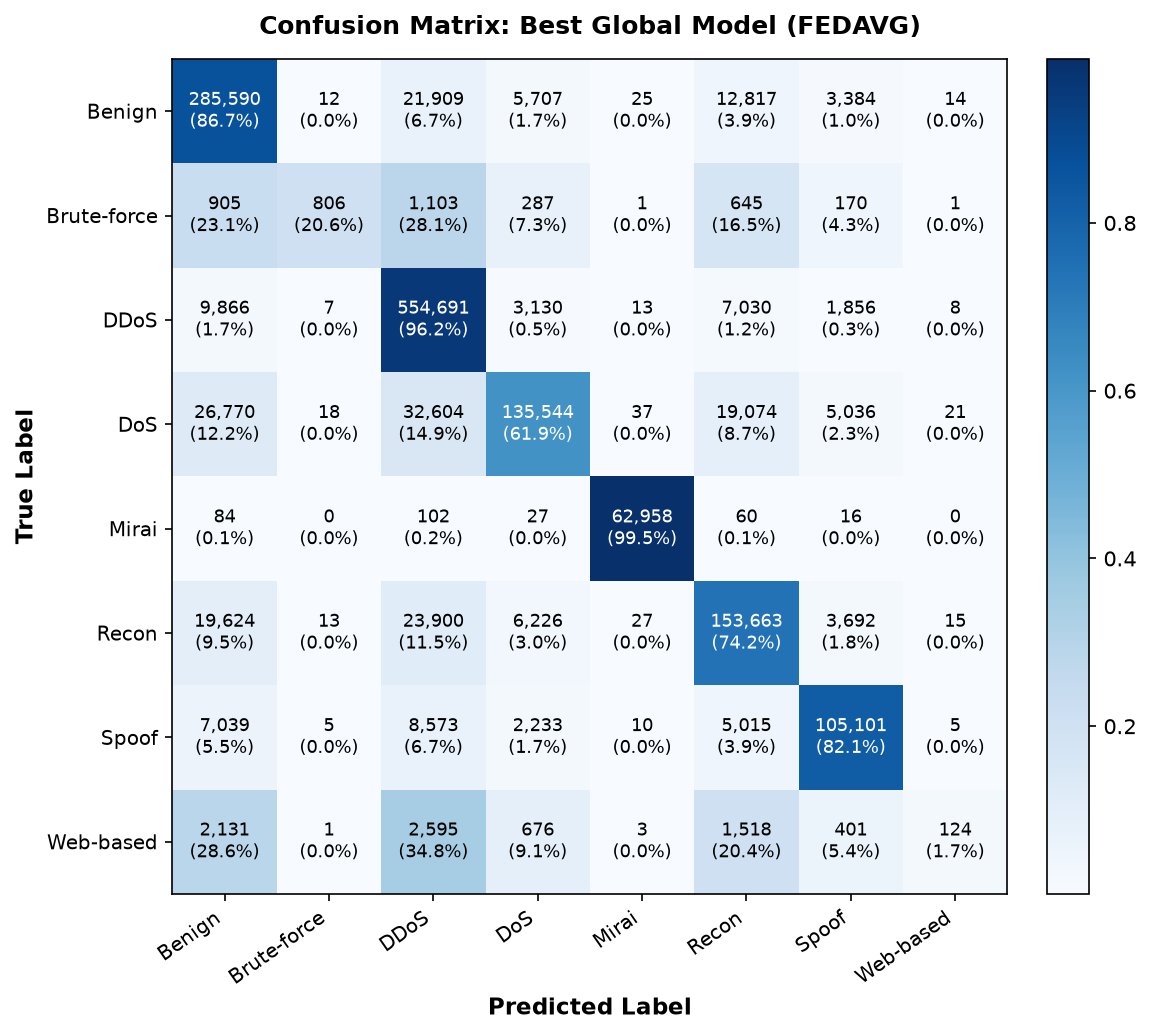
\includegraphics[width=\textwidth]{figures/cm_e2_fedavg.png}
        \caption{Ma trận nhầm lẫn 8x8 (E2 FedAvg IID).}
        \label{fig:cm_e2}
    \end{subfigure}
    \hfill
    \begin{subfigure}[b]{0.48\textwidth}
        \centering
        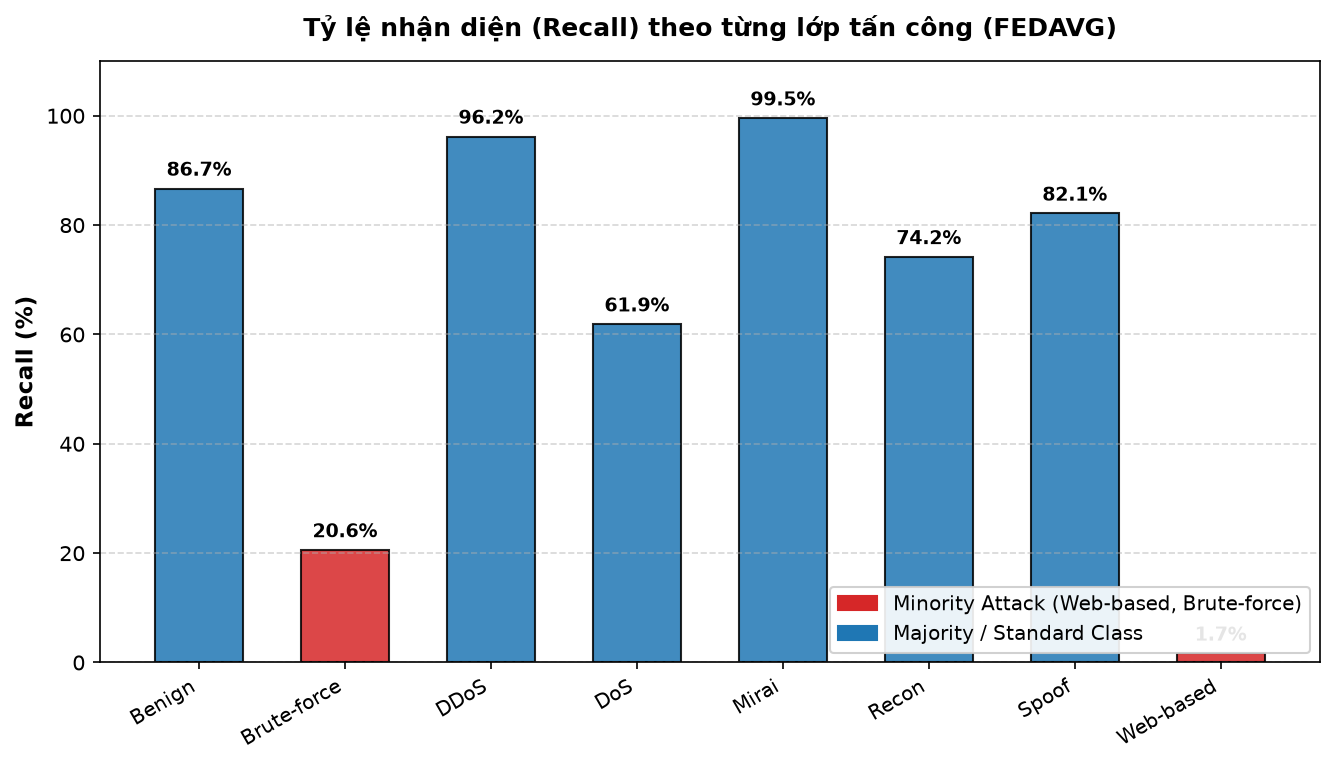
\includegraphics[width=\textwidth]{figures/recall_e2_fedavg.png}
        \caption{Tỷ lệ Recall theo lớp (E2 FedAvg IID).}
        \label{fig:recall_e2}
    \end{subfigure}
    \caption{Trực quan hóa ma trận nhầm lẫn chuẩn hóa và tỷ lệ Recall theo từng lớp tấn công.}
    \label{fig:cm_recall}
\end{figure}

\subsubsection{Phát hiện 2: Đường cong Suy thoái Định lượng theo Hệ số Dirichlet $\alpha$}
Khi quan sát sự dịch chuyển của FedAvg và FedProx từ IID sang Non-IID:
\begin{itemize}
    \item \textbf{Độ trôi tham số (Drift L2 Norm):} Ở FedAvg, khi $\alpha$ giảm từ $1.0$ xuống $0.5$, độ trôi tăng từ $10.75$ lên $13.30$ ($+23.7\%$). Ngược lại, FedProx kiểm soát độ trôi cực kỳ nghiêm ngặt, luôn duy trì L2 norm dưới $0.65$ (giảm hơn $95\%$ so với FedAvg).
    \item \textbf{Suy thoái Macro-F1:} Mặc dù FedProx kiểm soát tốt độ trôi, Macro-F1 vẫn sụt giảm từ $59.06\%$ (E2) xuống $43.01\%$ (E5, $\alpha=0.1$). Điều này chứng minh rằng việc giữ trọng số gần với mô hình toàn cục không thể bù đắp được việc thiếu hụt thông tin phân phối khi dữ liệu bị phân mảnh cực đoan.
\end{itemize}

\begin{figure}[H]
    \centering
    \begin{subfigure}[b]{0.48\textwidth}
        \centering
        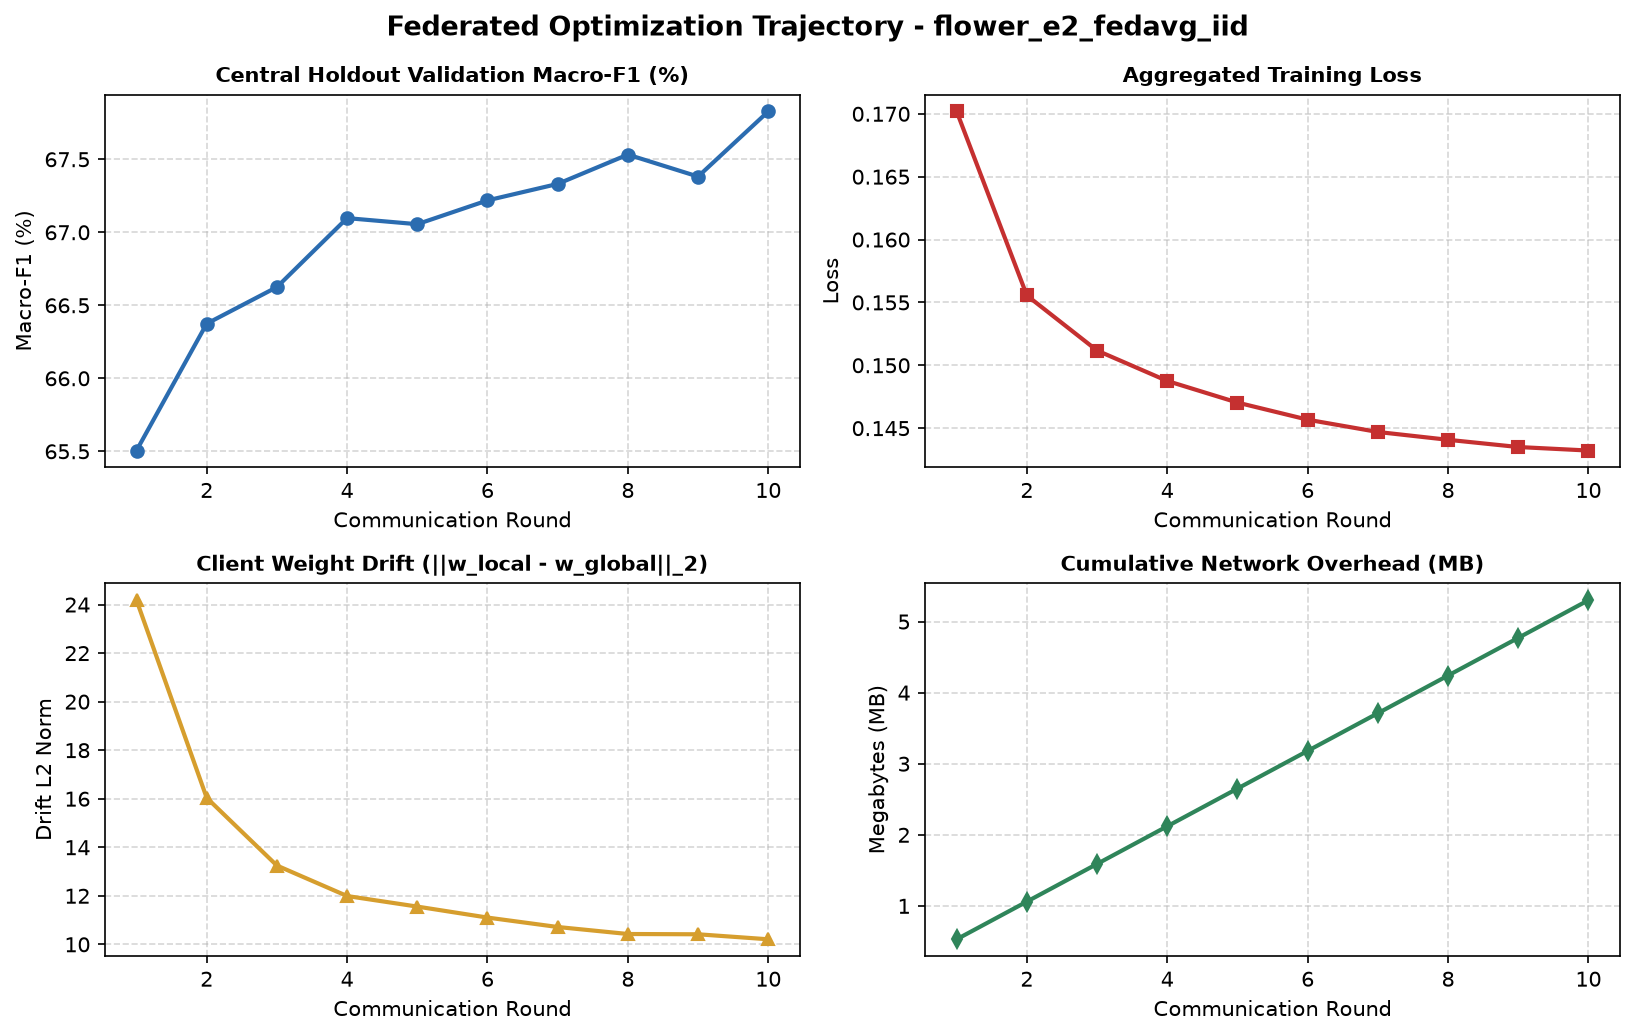
\includegraphics[width=\textwidth]{figures/conv_e2_fedavg.png}
        \caption{Quỹ đạo hội tụ $K=5$ (E2 FedAvg).}
        \label{fig:conv_e2}
    \end{subfigure}
    \hfill
    \begin{subfigure}[b]{0.48\textwidth}
        \centering
        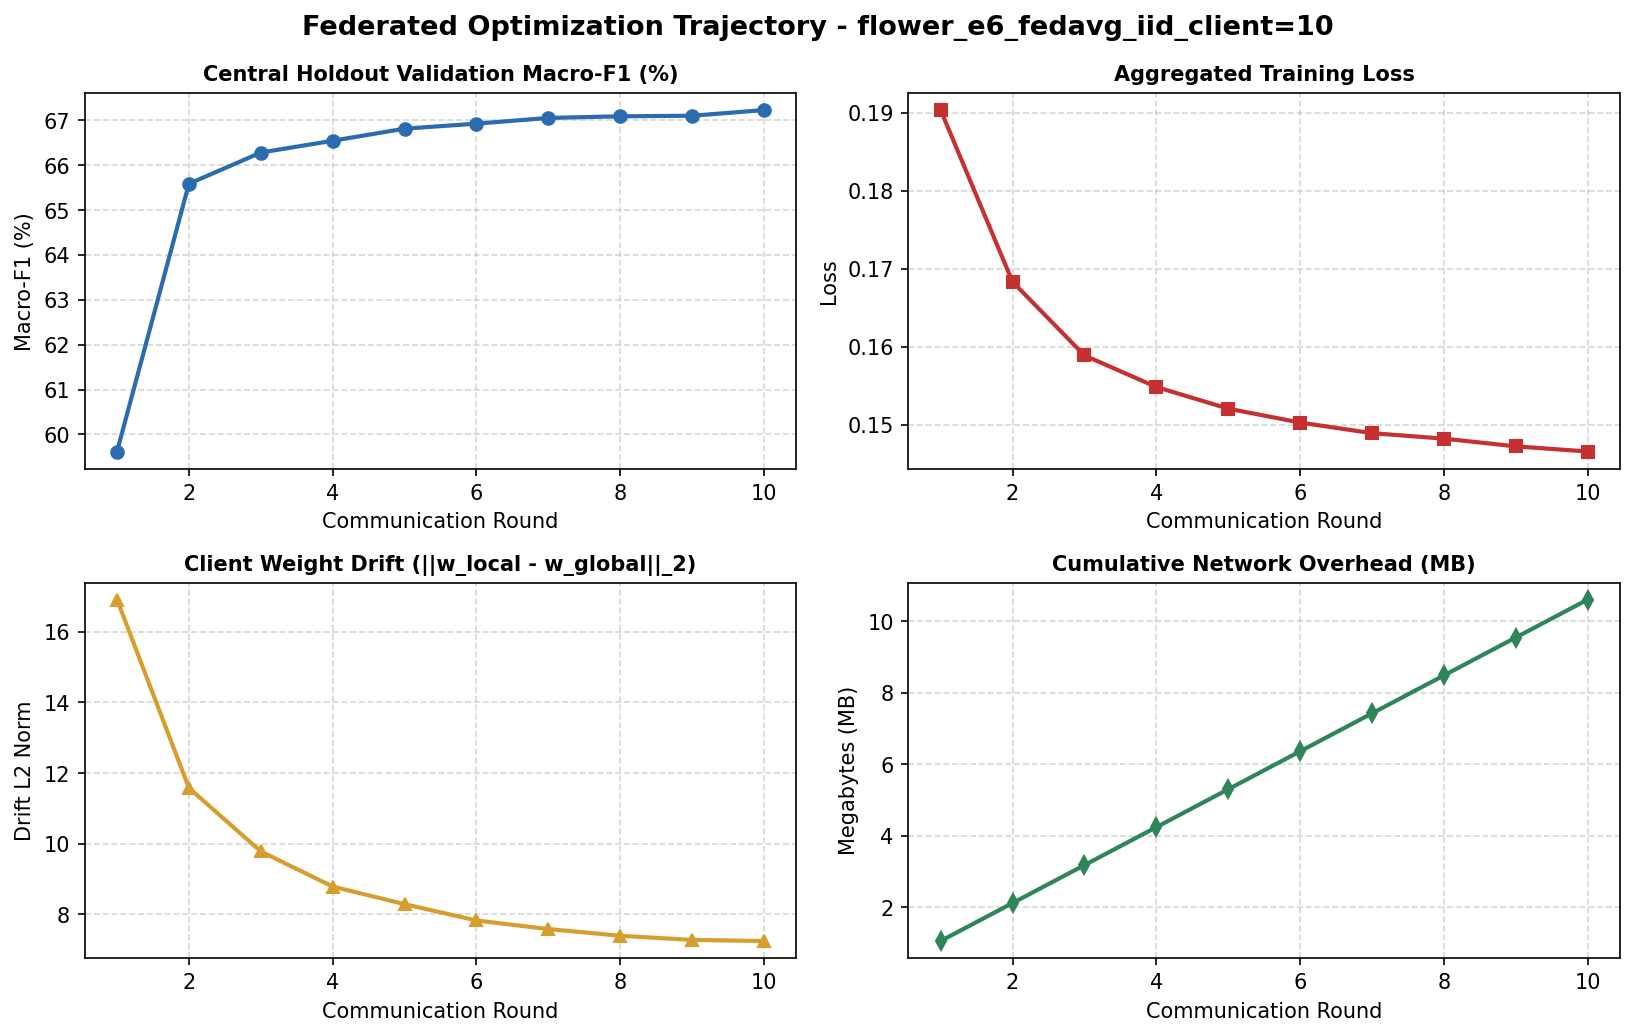
\includegraphics[width=\textwidth]{figures/conv_e6_10clients.png}
        \caption{Quỹ đạo hội tụ $K=10$ (E6 FedAvg).}
        \label{fig:conv_e6}
    \end{subfigure}
    \caption{Quỹ đạo hội tụ Macro-F1 và chi phí truyền thông tích lũy qua 10 rounds.}
    \label{fig:convergence}
\end{figure}

\subsubsection{Phát hiện 3: Tính Bền vững Mở rộng Quy mô (Scalability) của FedAvg}
Kịch bản E6 chứng minh rằng trong môi trường IID:
\begin{itemize}
    \item Khi số trạm biên tăng gấp đôi từ $K=5 \to 7 \to 10$, Macro-F1 duy trì độ ổn định ấn tượng: $68.00\% \to 67.82\% \to 67.28\%$ (mức độ suy thoái chỉ vỏn vẹn $0.72\%$).
    \item Chi phí truyền thông tích lũy tuân theo đúng hàm tuyến tính: $5.30\text{ MB} \to 7.42\text{ MB} \to 10.60\text{ MB}$. Kết quả này khẳng định tính khả thi vượt trội của kiến trúc Tabular MLP trên mạng biên IoT.
\end{itemize}

% ==============================================================================
% CHƯƠNG 5
% ==============================================================================
\section{Thảo luận, Hạn chế và Kế hoạch Tiếp theo}
\label{sec:discussion}

\subsection{Nhìn nhận Khách quan về các Hạn chế}
Như một nghiên cứu khoa học nghiêm túc, đề tài thừa nhận thẳng thắn ba hạn chế chính:
\begin{enumerate}
    \item \textbf{Điểm mù đối với tấn công Web-based:} Hệ thống chưa thể vận hành như một NIDS độc lập trong môi trường sản xuất nếu thiếu sự hỗ trợ của các giải pháp truyền thống (như Web Application Firewall -- WAF).
    \item \textbf{Giới hạn của môi trường mô phỏng:} Mặc dù sử dụng socket gRPC đa tiến trình thực tế, các thử nghiệm vẫn vận hành trên cùng một máy chủ vật lý, chưa tính đến độ trễ truyền sóng và hiện tượng rớt gói của mạng không dây IoT thực tế.
    \item \textbf{Phụ thuộc vào một tập dữ liệu đơn lẻ:} Toàn bộ phát hiện thực nghiệm được kiểm chứng trên CICIoT2023, cần thêm dữ liệu từ các bộ benchmark khác (như Edge-IIoTset hay TON\_IoT) để mở rộng tính tổng quát.
\end{enumerate}

\subsection{Kế hoạch Hoàn thiện Khóa luận}
Để hoàn thành $100\%$ khối lượng khóa luận tốt nghiệp theo đúng tiến độ:
\begin{itemize}
    \item Hoàn thành nốt kịch bản E1 (Centralized MLP Baseline) và E5 với FedAvg ($\alpha=0.1$) để khép kín bảng đối chứng.
    \item Mở rộng nội dung chi tiết của bản thảo LaTeX này thành cuốn Khóa luận hoàn chỉnh theo đúng định dạng quy định của Trường Đại học Công nghệ Thông tin.
    \item Xây dựng Slide thuyết trình và kịch bản demo thực nghiệm để bảo vệ trước Hội đồng.
\end{itemize}

% ==============================================================================
% TÀI LIỆU THAM KHẢO
% ==============================================================================
\bibliographystyle{IEEEtran}
\bibliography{references}

\end{document}
